\documentclass{article}

\usepackage{fancyhdr}
\usepackage{extramarks}
\usepackage{amsmath}
\usepackage{amsthm}
\usepackage{amsfonts}
\usepackage{tikz}
\usepackage[plain]{algorithm}
\usepackage{algpseudocode}
\usepackage{listings} 
\usepackage{neuralnetwork}
\usepackage{subfigure}
\usetikzlibrary{automata,positioning}

\usepackage{color}

\definecolor{dkgreen}{rgb}{0,0.6,0}
\definecolor{gray}{rgb}{0.5,0.5,0.5}
\definecolor{mauve}{rgb}{0.58,0,0.82}

\lstset{frame=tb,
  language=Python,
  aboveskip=3mm,
  belowskip=3mm,
  showstringspaces=false,
  columns=flexible,
  basicstyle={\small\ttfamily},
  numbers=none,
  numberstyle=\tiny\color{gray},
  keywordstyle=\color{blue},
  commentstyle=\color{dkgreen},
  stringstyle=\color{mauve},
  breaklines=true,
  breakatwhitespace=true,
  tabsize=3
}
%
% Basic Document Settings
%

\topmargin=-0.45in
\evensidemargin=0in
\oddsidemargin=0in
\textwidth=6.5in
\textheight=9.0in
\headsep=0.25in

\linespread{1.1}

\pagestyle{fancy}
\lhead{\hmwkAuthorName}
\chead{\hmwkClass\: \hmwkTitle}
\rhead{\firstxmark}
\lfoot{\lastxmark}
\cfoot{\thepage}

\renewcommand\headrulewidth{0.4pt}
\renewcommand\footrulewidth{0.4pt}

\setlength\parindent{0pt}

%
% Create Problem Sections
%

\newcommand{\enterProblemHeader}[1]{
    \nobreak\extramarks{}{Task \arabic{#1} continued on next page\ldots}\nobreak{}
    \nobreak\extramarks{Task \arabic{#1} (continued)}{Problem \arabic{#1} continued on next page\ldots}\nobreak{}
}

\newcommand{\exitProblemHeader}[1]{
    \nobreak\extramarks{Task \arabic{#1} (continued)}{Problem \arabic{#1} continued on next page\ldots}\nobreak{}
    \stepcounter{#1}
    \nobreak\extramarks{Task \arabic{#1}}{}\nobreak{}
}

\setcounter{secnumdepth}{0}
\newcounter{partCounter}
\newcounter{homeworkProblemCounter}
\setcounter{homeworkProblemCounter}{1}
\nobreak\extramarks{Task \arabic{homeworkProblemCounter}}{}\nobreak{}

%
% Homework Problem Environment
%
% This environment takes an optional argument. When given, it will adjust the
% problem counter. This is useful for when the problems given for your
% assignment aren't sequential. See the last 3 problems of this template for an
% example.
%
\newenvironment{homeworkProblem}[1][-1]{
    \ifnum#1>0
        \setcounter{homeworkProblemCounter}{#1}
    \fi
    \section{Task \arabic{homeworkProblemCounter}}
    \setcounter{partCounter}{1}
    \enterProblemHeader{homeworkProblemCounter}
}{
    \exitProblemHeader{homeworkProblemCounter}
}

%
% Homework Details
%   - Title
%   - Due date
%   - Class
%   - Section/Time
%   - Instructor
%   - Author
%

\newcommand{\hmwkTitle}{Assignment\ \#1}
\newcommand{\hmwkDueDate}{March 10, 2019}
\newcommand{\hmwkClass}{CSCI964 Computational Intelligence}
\newcommand{\hmwkClassTime}{2.14}
\newcommand{\hmwkClassInstructor}{Zhifeng Wang}
\newcommand{\hmwkAuthorName}{\textbf{Mei Wangzhihui}}
\newcommand{\hmwkAuthorNum}{\textbf{2019124044}}
%
% Title Page
%

\title{
    \vspace{2in}
    \textmd{\textbf{\hmwkClass:\ \hmwkTitle}}\\
    % \normalsize\vspace{0.1in}\small{Due\ on\ \hmwkDueDate\ at 3:10pm}\\
    % \vspace{0.1in}\large{\textit{\hmwkClassInstructor\ \hmwkClassTime}}
    \vspace{3in}
}

\author{\hmwkAuthorName\ \hmwkAuthorNum}
\date{}

\renewcommand{\part}[1]{\textbf{\large Part \Alph{partCounter}}\stepcounter{partCounter}\\}

%
% Various Helper Commands
%

% Useful for algorithms
\newcommand{\alg}[1]{\textsc{\bfseries \footnotesize #1}}

% For derivatives
\newcommand{\deriv}[1]{\frac{\mathrm{d}}{\mathrm{d}x} (#1)}

% For partial derivatives
\newcommand{\pderiv}[2]{\frac{\partial}{\partial #1} (#2)}

% Integral dx
\newcommand{\dx}{\mathrm{d}x}

% Alias for the Solution section header
\newcommand{\solution}{\textbf{\large Solution}}

% Probability commands: Expectation, Variance, Covariance, Bias
\newcommand{\E}{\mathrm{E}}
\newcommand{\Var}{\mathrm{Var}}
\newcommand{\Cov}{\mathrm{Cov}}
\newcommand{\Bias}{\mathrm{Bias}}

\begin{document}

\maketitle

\pagebreak

\begin{homeworkProblem}
  The \textbf{two-spiral problem} is a two class problem, which is non-linear.
  \begin{figure}[H]
    \centering
    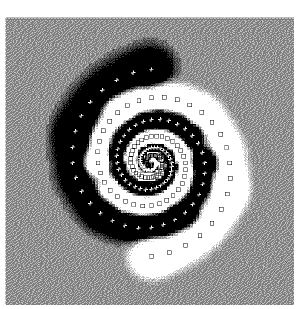
\includegraphics[width=0.5\textwidth]{image/d1}
    \caption{two-spiral problem}
\end{figure}
  I use a 2-layer MLP to solve this problem as the problem is non-linear. 
  First I try to use a single-hidden-layer to fit the problem.
  But the graph fluctuate heavily. I try to turn down the learning rate(LR) and turn up the momentum (Mtm) so that it can converange more smoothly. But the wrong rate is high.
  \begin{figure}[H]
      \centering
      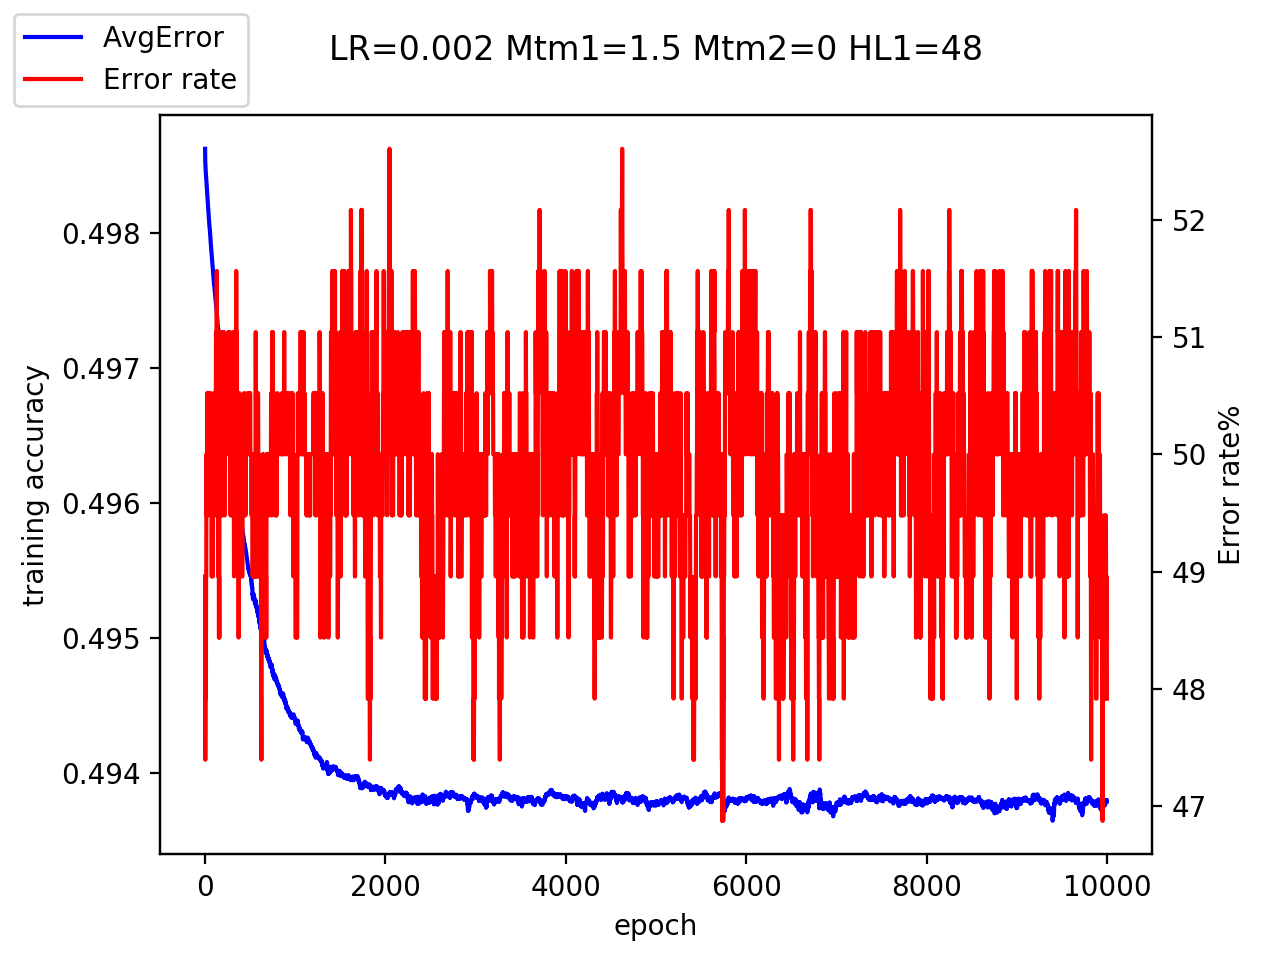
\includegraphics[width=0.6\textwidth]{image/d1ff1}
      \caption{3-layer MLP}
  \end{figure}
  The I add one hidden layer to solve it. 
  \begin{figure}[H]
    \centering
    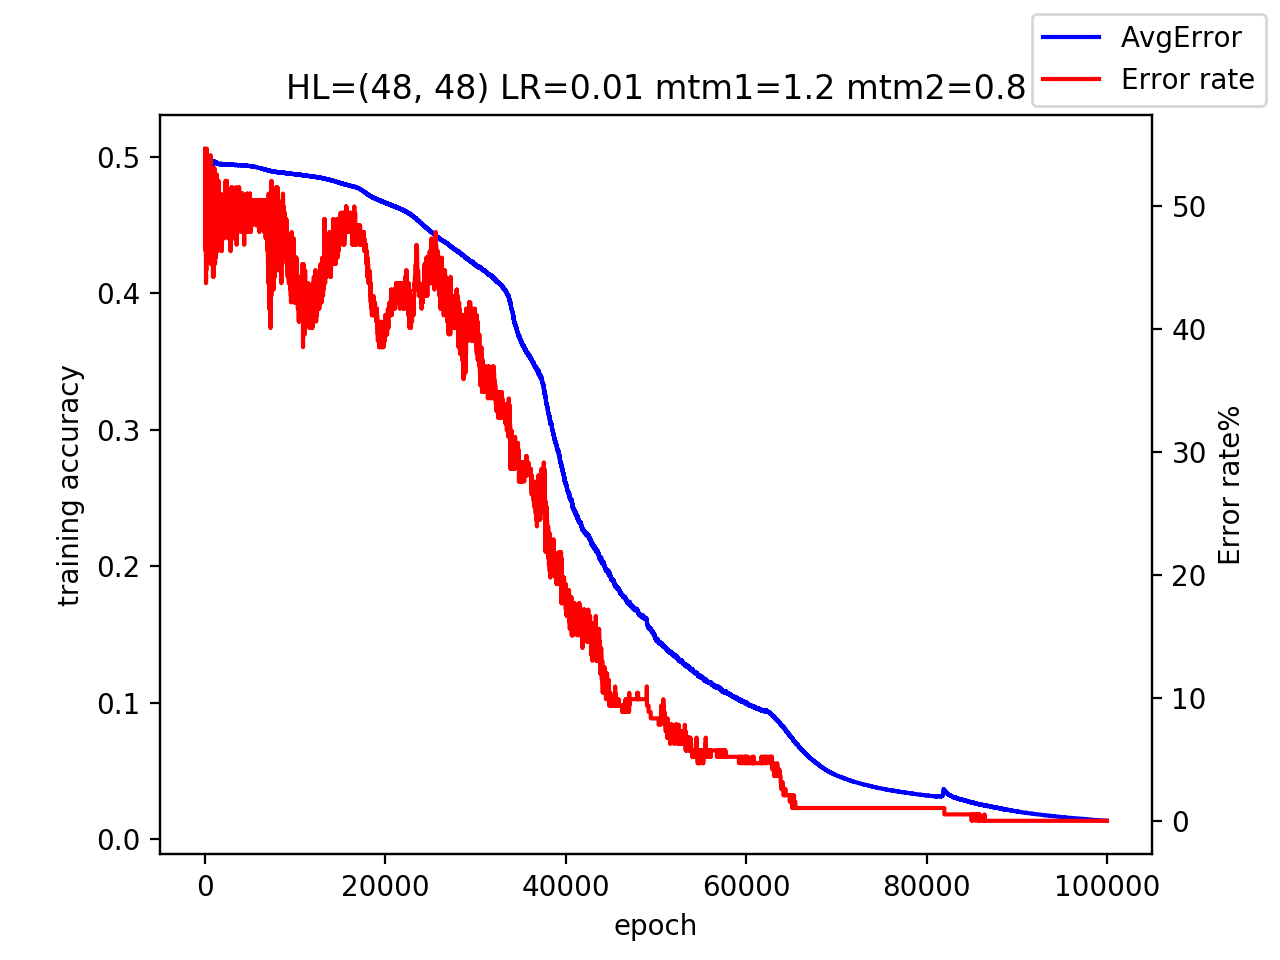
\includegraphics[width=0.6\textwidth]{image/d1f2}
    \caption{4-layer MLP}
\end{figure}
The model applied on test dataset is : AvgError = 0.001843, Error rate = 0.82\%. Generally, It's a good model. But the performance is not optimized.

Adding an extra layer into it:
\begin{figure}[H]
  \centering
  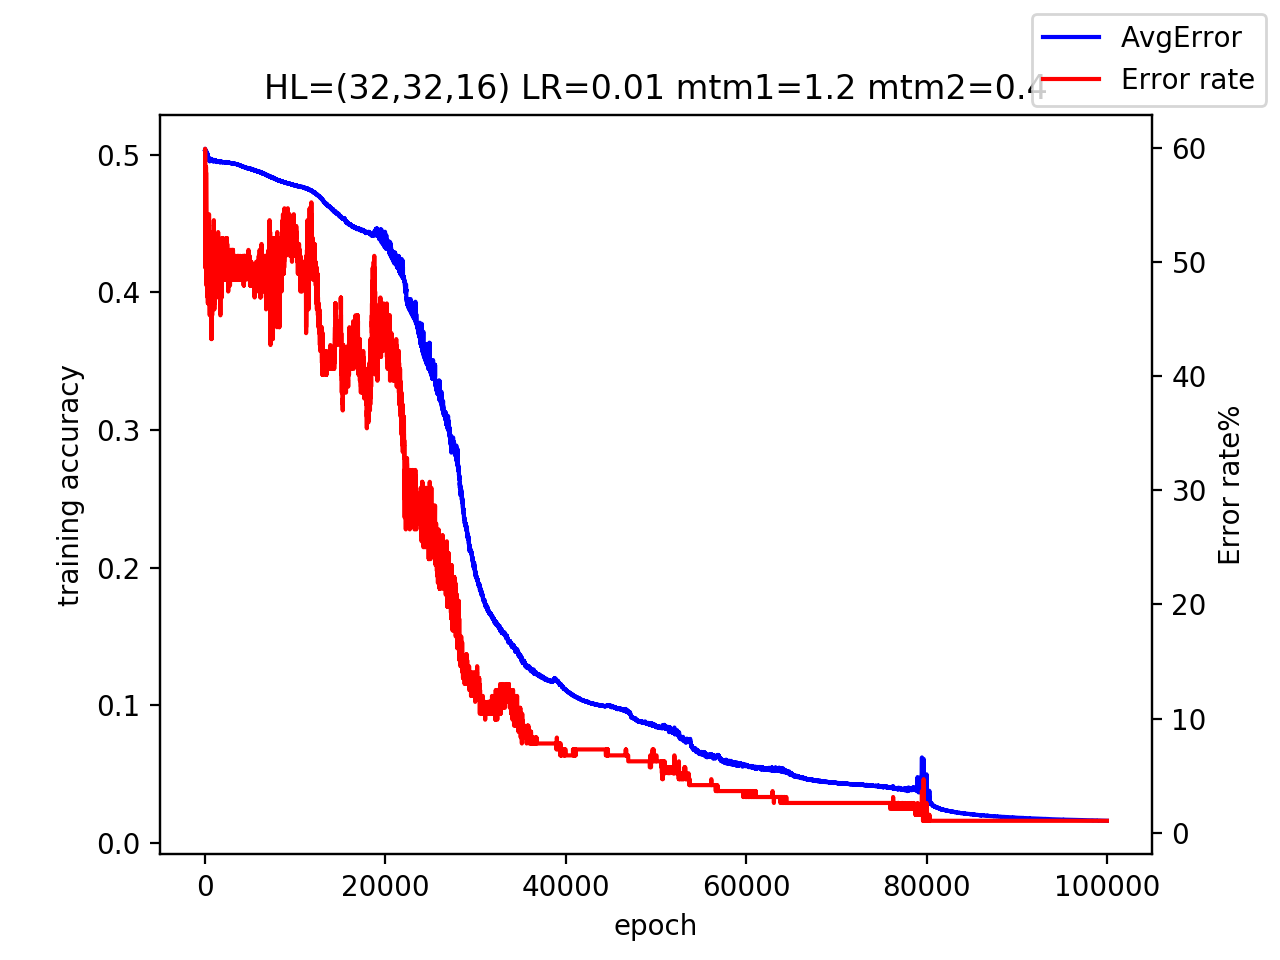
\includegraphics[width=0.6\textwidth]{image/d1f1}
  \caption{5-layer MLP}
\end{figure}
For Test Set $AvgError=0.0028466$ and  $ Error rate= 1.56\%$
\end{homeworkProblem}
though it predict weeker than the second MLP, but it perform better in computation complexisity.
\clearpage
\begin{homeworkProblem}
  \textbf{1-hidden-layer MLP}
  \begin{figure}[H]
    \centering
    \subfigure[fig1.]{
      \begin{minipage}[t]{0.5\linewidth}
      \centering
      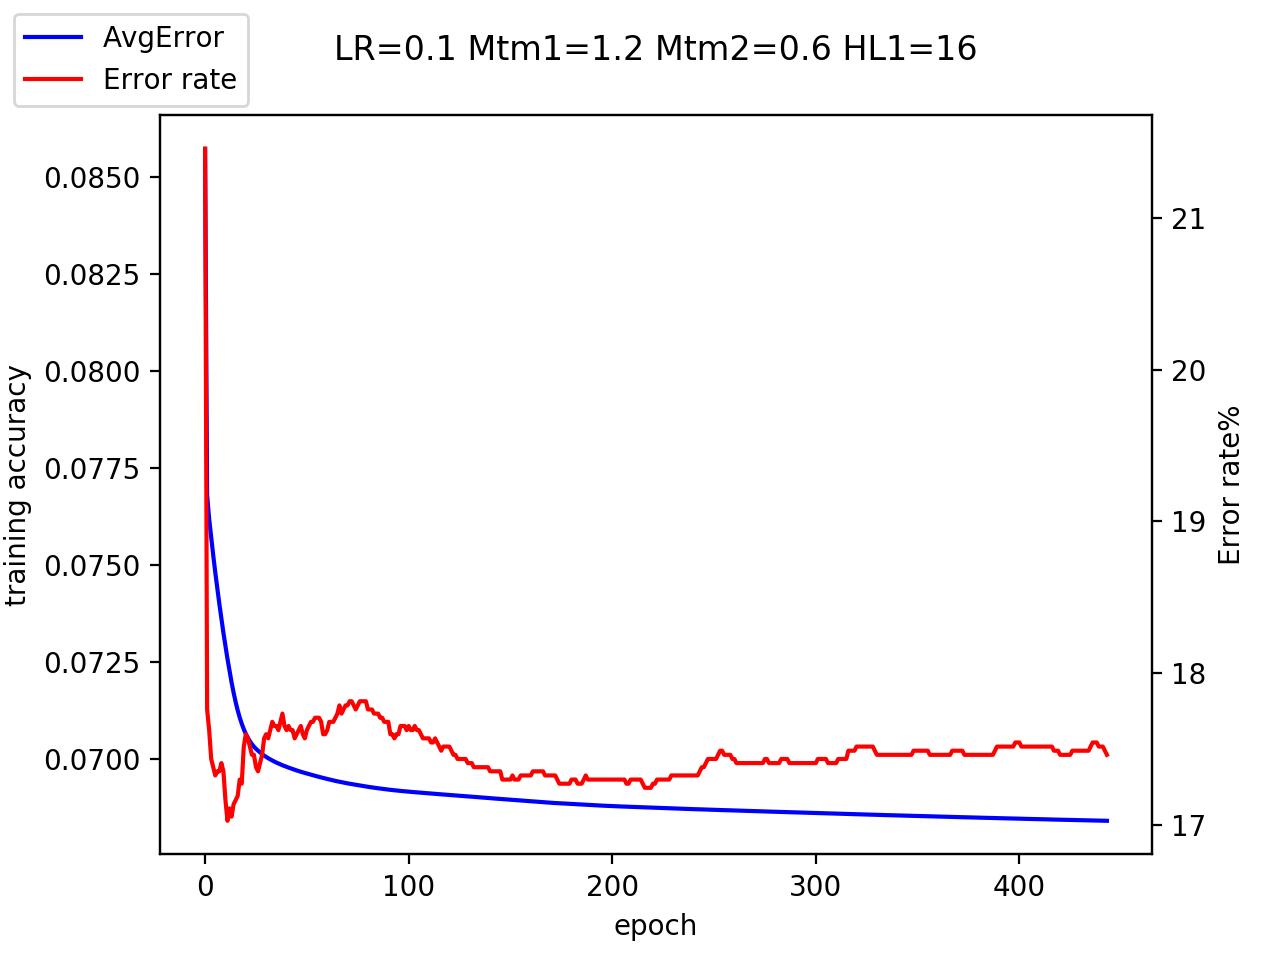
\includegraphics[width=3in]{image/d2f1}
      \end{minipage}% 
      }%
      \subfigure[fig2.]{
        \begin{minipage}[t]{0.5\linewidth}
        \centering
        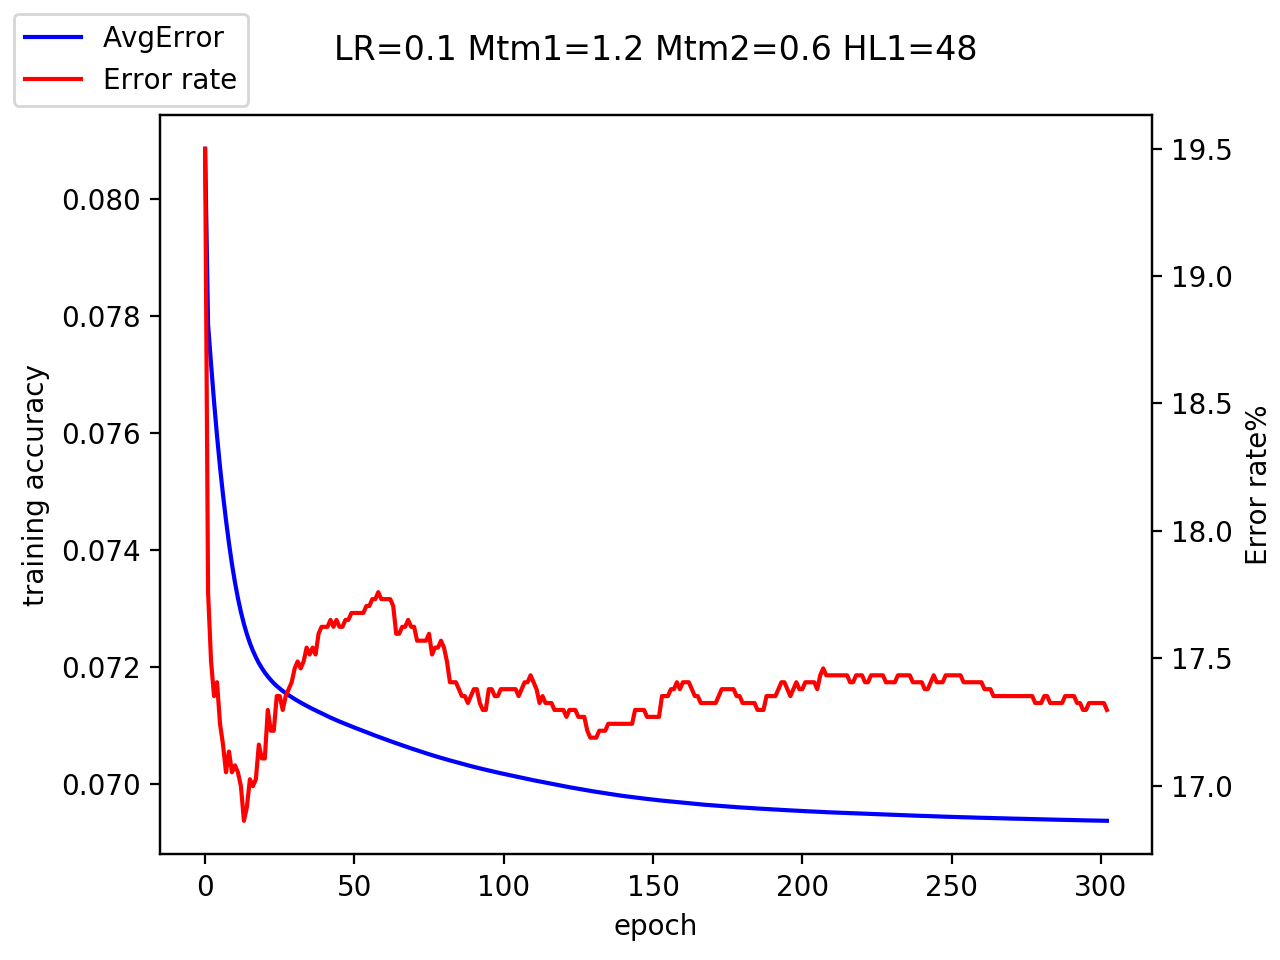
\includegraphics[width=3in]{image/d2f3}
        \end{minipage}% 
        }%
      \\
      \subfigure[fig3.]{
        \begin{minipage}[t]{0.5\linewidth}
        \centering
        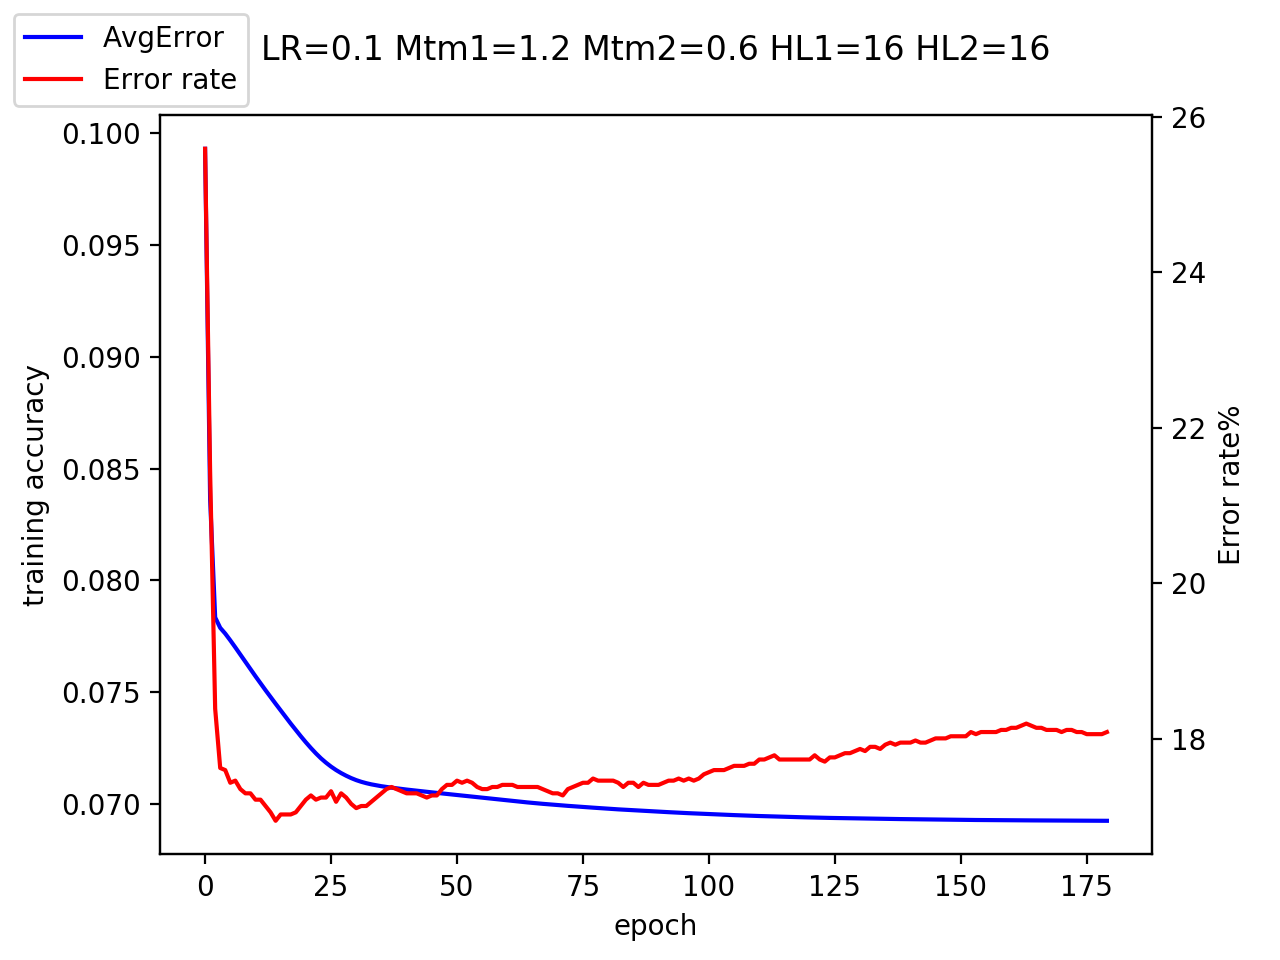
\includegraphics[width=3in]{image/d2f4}
        \end{minipage}% 
      }% 
      \subfigure[fig4.]{
        \begin{minipage}[t]{0.5\linewidth}
        \centering
        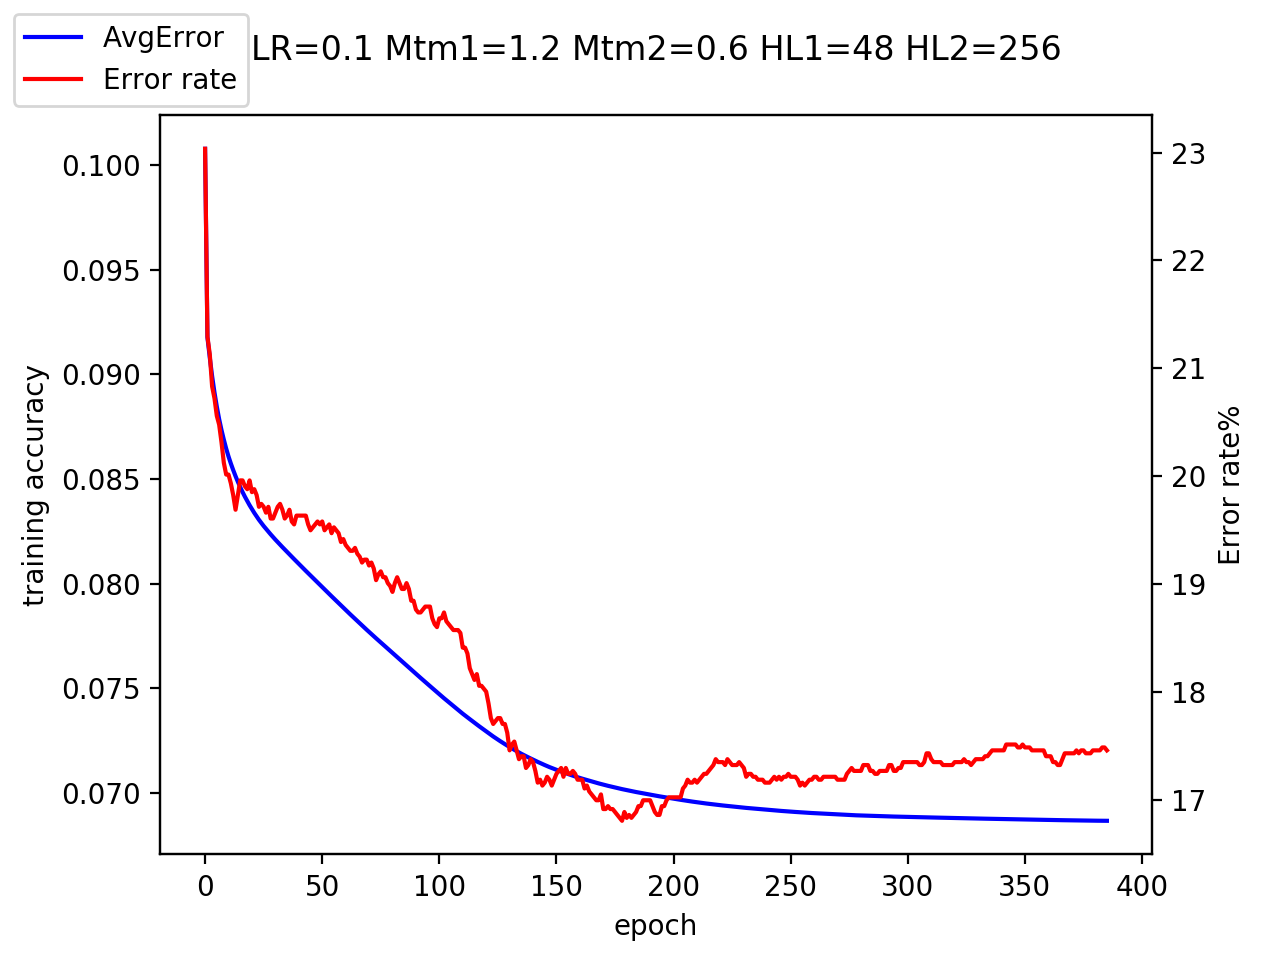
\includegraphics[width=3in]{image/d2f6}
        \end{minipage}% 
      }%
      \\
      \subfigure[fig5.]{
        \begin{minipage}[t]{0.5\linewidth}
        \centering
        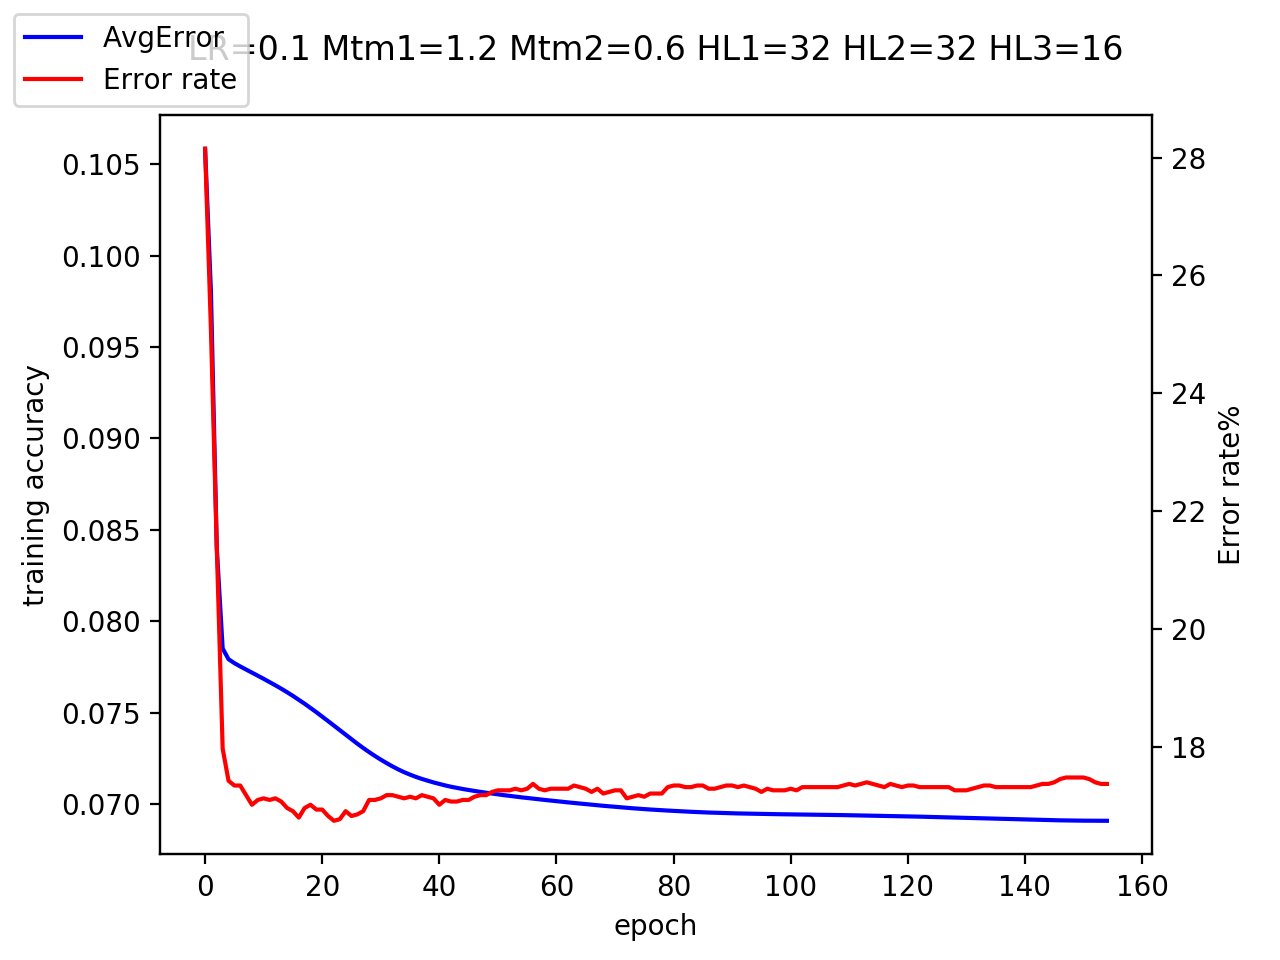
\includegraphics[width=3in]{image/d2f8}
        \end{minipage}% 
      }%
      \subfigure[fig6.]{
        \begin{minipage}[t]{0.5\linewidth}
        \centering
        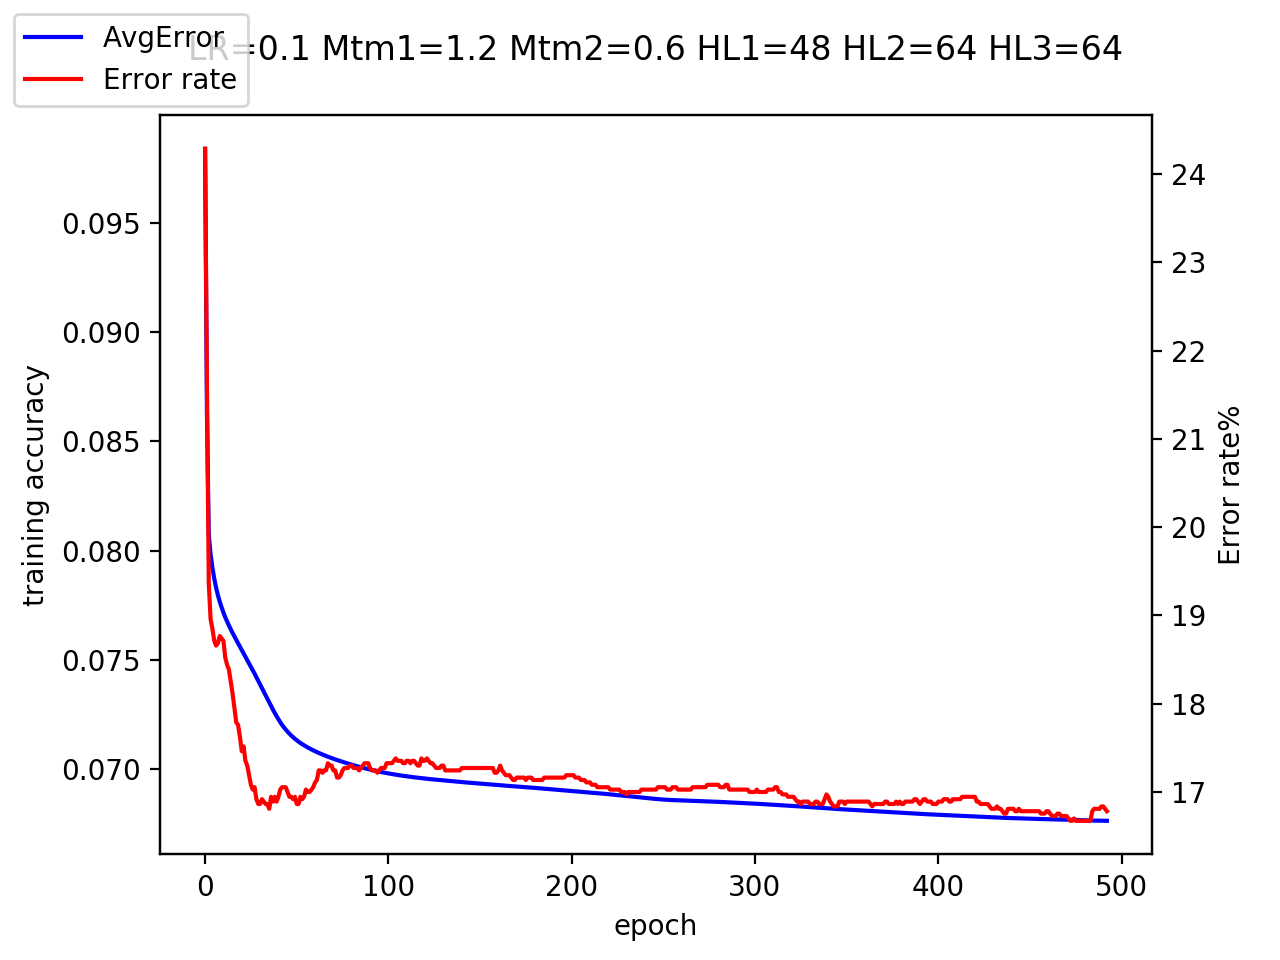
\includegraphics[width=3in]{image/d2f10}
        \end{minipage}% 
      }%
     
    \caption{MLP}
  \end{figure} 

  The performance of these MLP is:
  \begin{table}[H]
    \centering
    \begin{tabular}{|l|l|l|l|}
    \hline
        Hidden Layer & Average Error & Error rate & Training Time \\ \hline
        16 & 0.071 & 0.23 & 5s \\ \hline
        48 & 0.075 & 0.238 & 16s \\ \hline
        16, 16 & 0.07 & 0.224 & 34s \\ \hline
        48, 256 & 0.072 & 0.238 & 273s \\ \hline
        32, 32, 16 & 0.071 & 0.226 & 158s \\ \hline
        48, 64, 64 & 0.070 & 0.224 & 213s \\ \hline
    \end{tabular}
    \caption{Performance of MLPs}
\end{table}
 With the consideration of the balance between Accuracy and performance, The 2-hidden-layer (16,16) is the best choice.
\end{homeworkProblem}
\begin{homeworkProblem}
  \begin{figure}[H]
    \centering
    \subfigure[fig1.]{
      \begin{minipage}[t]{0.5\linewidth}
      \centering
      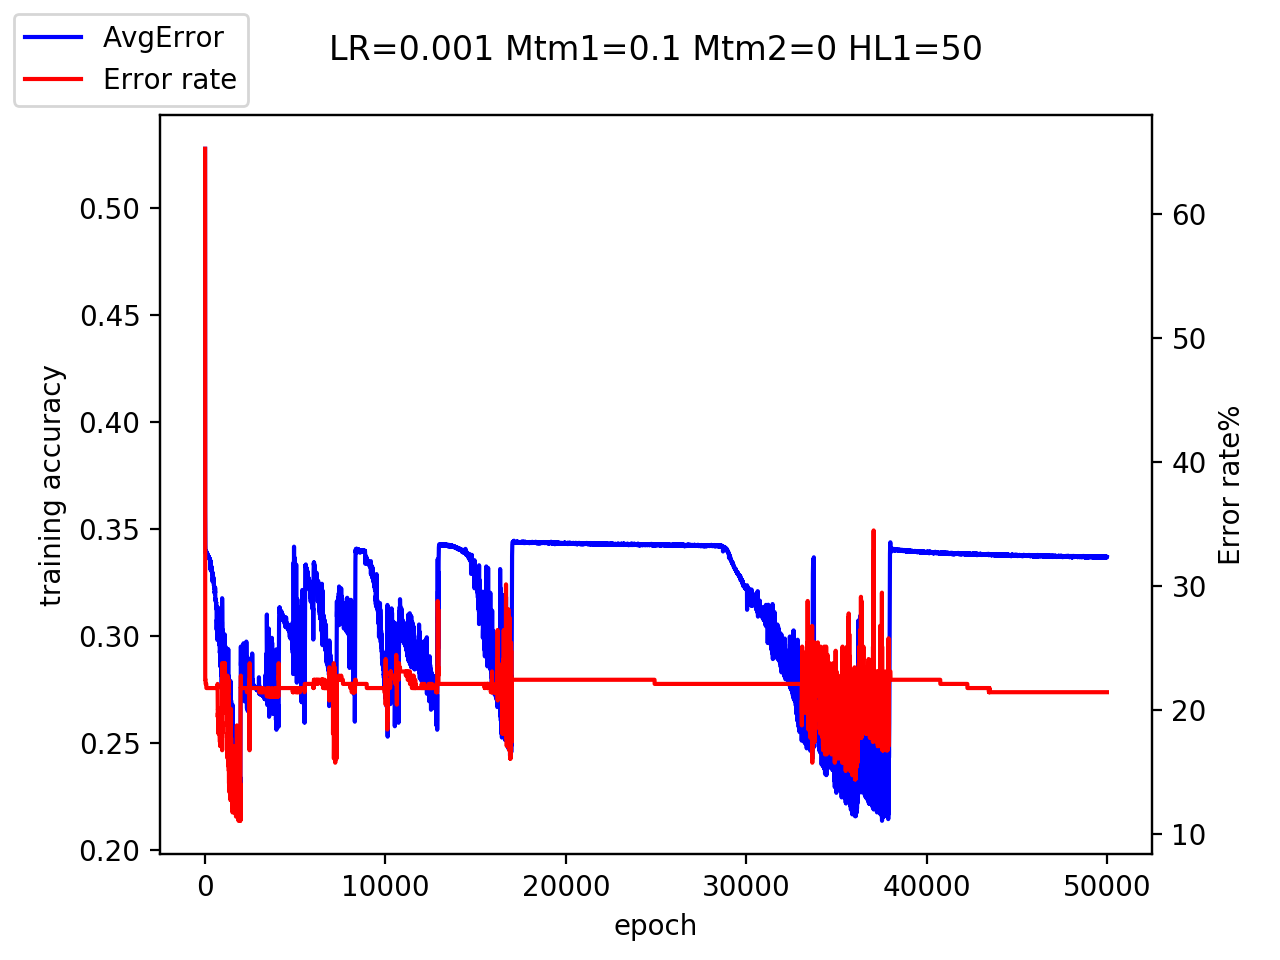
\includegraphics[width=3in]{image/d3ff1}
      \end{minipage}% 
      }%
      \subfigure[fig2.]{
        \begin{minipage}[t]{0.5\linewidth}
        \centering
        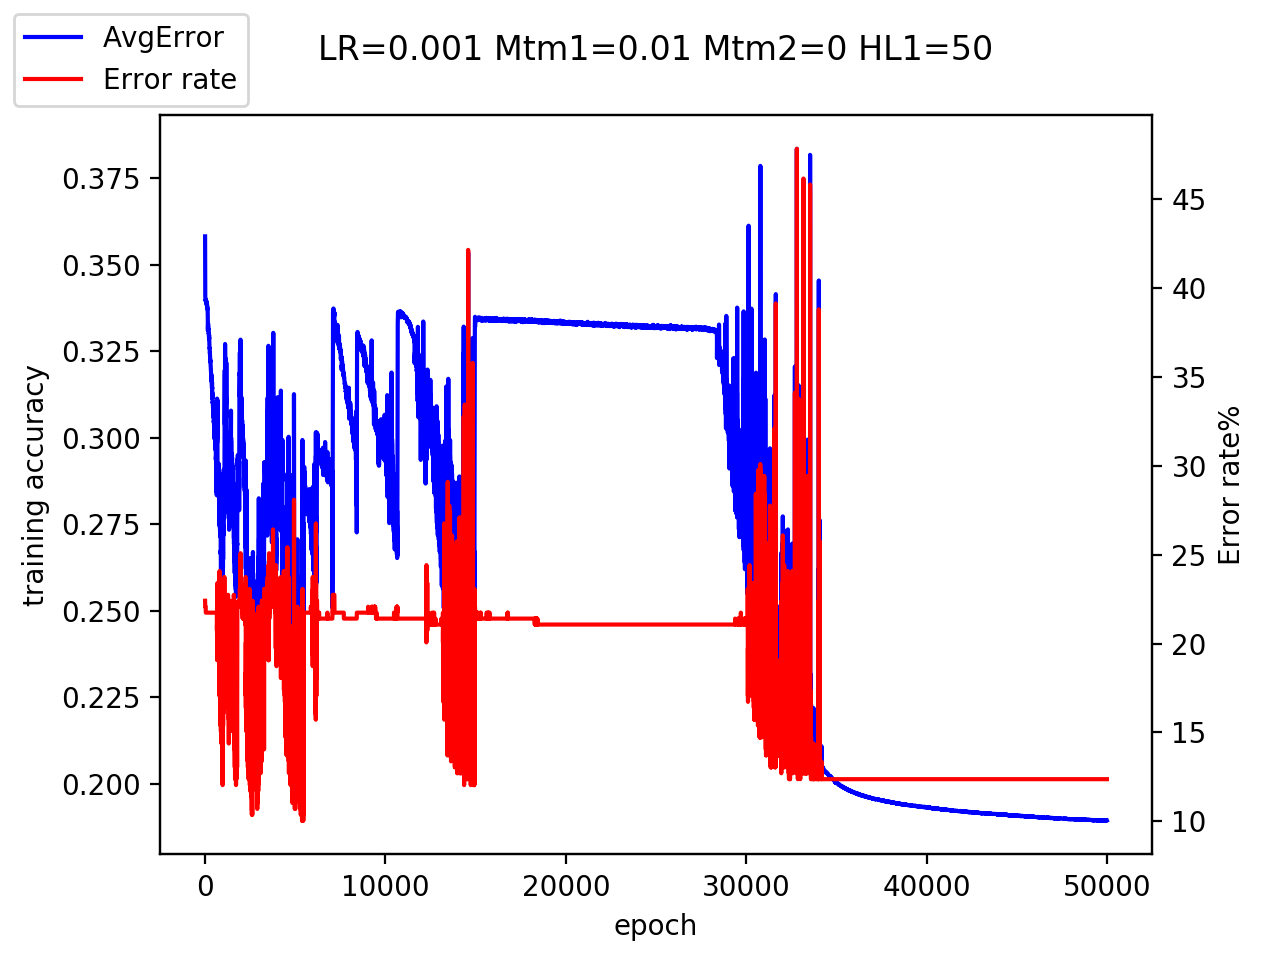
\includegraphics[width=3in]{image/d3ff2}
        \end{minipage}% 
        }%
      \\
    \caption{bad example}
  \end{figure}
  \begin{figure}[H]
    \centering
    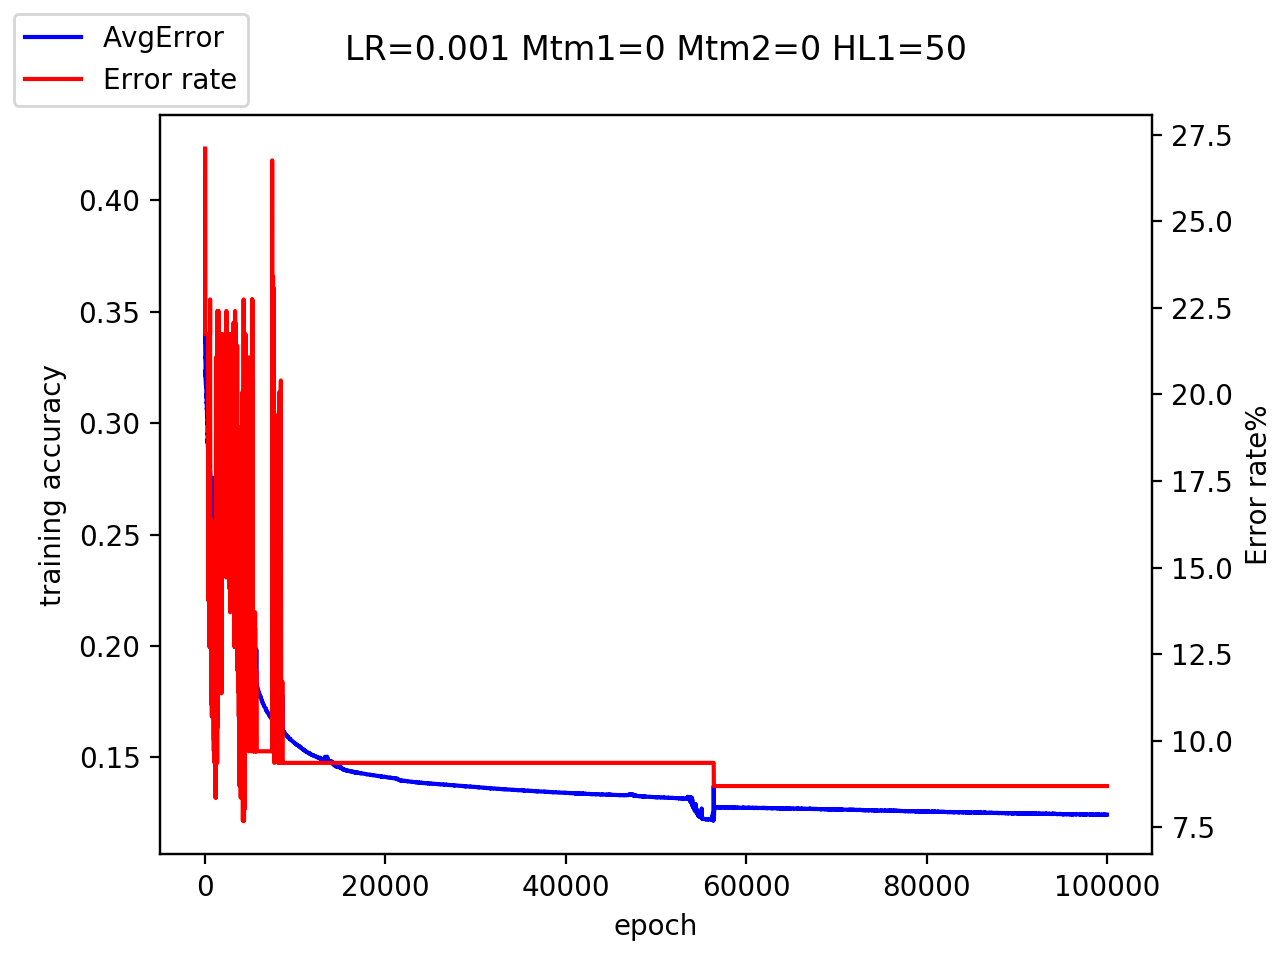
\includegraphics[width=3in]{image/d3f1}
    \caption{MLP with 1-hidden layer}
  \end{figure}
  The final $Average Error = 0.205$ and $ Error Rate = 4\%$, The time to converange the MLP is 100000 epochs.
\end{homeworkProblem}
\end{document}
